\documentclass[12pt,]{article}
\usepackage{lmodern}
\usepackage{amssymb,amsmath}
\usepackage{ifxetex,ifluatex}
\usepackage{fixltx2e} % provides \textsubscript
\ifnum 0\ifxetex 1\fi\ifluatex 1\fi=0 % if pdftex
  \usepackage[T1]{fontenc}
  \usepackage[utf8]{inputenc}
\else % if luatex or xelatex
  \ifxetex
    \usepackage{mathspec}
    \usepackage{xltxtra,xunicode}
  \else
    \usepackage{fontspec}
  \fi
  \defaultfontfeatures{Mapping=tex-text,Scale=MatchLowercase}
  \newcommand{\euro}{€}
\fi
% use upquote if available, for straight quotes in verbatim environments
\IfFileExists{upquote.sty}{\usepackage{upquote}}{}
% use microtype if available
\IfFileExists{microtype.sty}{%
\usepackage{microtype}
\UseMicrotypeSet[protrusion]{basicmath} % disable protrusion for tt fonts
}{}
\usepackage[margin=1in]{geometry}
\usepackage{longtable,booktabs}
\ifxetex
  \usepackage[setpagesize=false, % page size defined by xetex
              unicode=false, % unicode breaks when used with xetex
              xetex]{hyperref}
\else
  \usepackage[unicode=true]{hyperref}
\fi
\hypersetup{breaklinks=true,
            bookmarks=true,
            pdfauthor={},
            pdftitle={},
            colorlinks=true,
            citecolor=blue,
            urlcolor=black,
            linkcolor=black,
            pdfborder={0 0 0}}
\urlstyle{same}  % don't use monospace font for urls
\setlength{\parindent}{0pt}
\setlength{\parskip}{6pt plus 2pt minus 1pt}
\setlength{\emergencystretch}{3em}  % prevent overfull lines
\setcounter{secnumdepth}{0}

%%% Use protect on footnotes to avoid problems with footnotes in titles
\let\rmarkdownfootnote\footnote%
\def\footnote{\protect\rmarkdownfootnote}

%%% Change title format to be more compact
\usepackage{titling}

% Create subtitle command for use in maketitle
\newcommand{\subtitle}[1]{
  \posttitle{
    \begin{center}\large#1\end{center}
    }
}

\setlength{\droptitle}{-2em}
  \title{}
  \pretitle{\vspace{\droptitle}}
  \posttitle{}
  \author{}
  \preauthor{}\postauthor{}
  \date{}
  \predate{}\postdate{}

\usepackage{lineno}
\usepackage{rotating}
\usepackage{times}
\usepackage{color, soul}
\usepackage{enumitem}
\usepackage[document]{ragged2e}
\usepackage[font={footnotesize},labelfont={sf,bf},labelsep=space]{caption}
\usepackage{titlesec}
\titleformat{\section}{\normalfont\fontsize{14}{15}\bfseries}{\thesection}{0 em}{}
\titleformat{\subsection}{\normalfont\fontsize{12}{15}\bfseries}{\thesubsection}{0 em}{}
\titlespacing{\section}{0pt}{\parskip}{-\lineskip}
\titlespacing{\subsection}{0pt}{\parskip}{-\parskip}


\begin{document}

\maketitle


\pagenumbering{roman}

\begin{description}

\item[Short title:]{Compensatory dynamics in space and time}
\item[Name:]{Andrew Tredennick}
\item[Contact information:] { ~\\
  email: atredenn@gmail.com \\
  phone: 970-443-1599}
\item[Date of Ph.D.:]{August 2014 (Colorado State University)} 

\end{description}

\newpage{}

\begin{center}
\large{\bf{Project Summary}}
\end{center}

\begin{description}
\item[Project Summary:]{
Ecosystems are intrinsically hierarchical, meaning that lower-level dynamics influence higher-level functioning.
For example, unique responses of populations and species to variable environmental conditions can buffer ecosystem-level function in space and time.
Understanding the degree to which such unique responses generate compensatory dynamics is key to understanding the consequences of climate change.
This project seeks to answer four questions motivated \textbf{Hypothesis H3} in the NWT LTER VII proposal: (1) Do compensatory dynamics contribute to ecosystem stability, and at what temporal and spatial scales? (2) What are the climate drivers of compensatory dynamics in space and time? (3) Will predicted climate change increase or decrease compensatory dynamics? And (4) Do opposing demographic responses to climate create compensatory dynamics among populations within species?
To answer these questions I will use several Niwot Ridge LTER vegetation data sets that are temporally and spatially replicated coupled with population modeling approaches.
Answering my questions will yield considerable insight into the dynamics of focal ecosystems at Niwot and advance our fundamental knowledge on the causes and consequences of compensatory dynamics.
Results from this project are also fundamental for testing \textbf{Hypthesis H4} in the NWT LTER VII proposal. 
}

\item[Keywords:]{\emph{synchrony, stability, portfolio effects, spatial insurance effect, climate}}

\item[Potential Conflicts of Interest:]{None.}
\end{description}

\newpage{}

\pagenumbering{arabic}

\begin{center}
\large{\bf{Research Proposal: Leveraging long-term data to understand the causes and consequences of compensatory dynamics in space and time}}
\end{center}

\setlength{\parindent}{0ex}

\section{Background}

What makes ecosystem functioning stable through time, or not, has
puzzled ecologists for decades and has profound implications for
ecosystem management in an increasingly variable world. It is now clear
that more species rich ecosystems tend to be more stable through time,
in part because of compensatory dynamics (Loreau and {{de Mazancourt}}
2013). Compensatory dynamics arise when species' fluctuations through
time are not in perfect synchrony, either as a result of interspecific
competition or species-specific responses to environmental conditions
(Loreau and {{de Mazancourt}} 2008, Gonzalez and Loreau 2009). Thus,
regardless of species richness, understanding the causes and
consequences of compensatory dynamics in natural ecosystems is essential
to understanding ecosystem stability. A mechanistic understanding of
compensatory dynamics is also necessary to predict how increasing
climate variability will impact the stability of ecosystem functioning.

For the past 30 years, research on ecosystem stability has focused on
the role of species fluctuations through time within local communities.
But across landscapes a hierarchical perspective reveals the importance
of compensatory dynamics among intraspecific populations, species, and
communities in space and time (Wang and Loreau 2014). For example, the
stability of aggregated ecosystem functioning depends on the synchrony
of local communities through time and the synchrony of species within
communities. Compensatory dynamics among local communities can arise
through species turnover (Wang and Loreau 2016) or populations
responding uniquely to environmental conditions because of demographic
trade-offs (Doak and Morris 2010). Such spatial dynamics are probably
strong drivers of ecosystem stability at the landscape scale, but we
know little about how important they are relative to within-community
temporal dynamics.

The goals of this project are to understand the causes and consequences
of compensatory dynamics across levels of spatial and ecological
organization. The Niwot Ridge Long Term Ecological Research (NWT)
station's ``saddle grid'' is an ideal system to gain this fundamental
understanding because it is spatially heterogenous, has a strong
environmental gradient across space (snow depth), there is species
turnover in space, and has long-term data that is necessary to estimate
temporal dynamics. I will use the long-term tundra vegetation data sets
and dynamic multispecies population models to attribute the buffering
effect of compensatory dynamics to specific machanisms in space and
time. The tight coupling of data and models will also allow me to
explore the impacts of realistic climate change scenarios on
compensatory dynamics and ecosystem stability.

\section{Research Questions}

This project is built around four questions motivated by
\textbf{Hypothesis H3} in the NWT LTER VII proposal: ``Asynchronous
responses to climate within one level of organization will combine to
reduce variability at a higher, aggregated, level. Climate change will
increase synchronicity through shared tolerance and growth
constraints.''

\begin{description}

\item[Q1.] \textbf{Do compensatory dynamics at lower-levels stabilize higher-level function?} Theory and experimental work shows that compensatory dynamics can stabilize ecosystem functioning through time, but the importance of compensatory dynamics in natural systems remains less understood. In particular, the role of spatial asynchrony, and what determines it, in stabilizing function as spatial scale increases is virtually unknown. To answer this question I will calculate and compare the variability of ecosystem functioning at multiple hierarchical levels (e.g., population, species, and community).

\item[Q2.] \textbf{What are the environmental drivers of observed compensatory dynamics?} The degree of compensatory dynamics is determined by how components respond to environmental conditions and how components interact. To answer this question I will fit dynamic multispecies population models with species-specific effects for climate covariates (e.g., snow depth and temperature).

\item[Q3.] \textbf{Will predicted climate change cause stability to increase or decrease through its affect on compensatory dynamics?} Depending on how components respond in space and time, synchrony could increase or decrease as the climate becomes more variable. To answer this question I simulate to multi-species model developed for Q2 under climate change scenarios of increasing means, variances, and both.

\item[Q4.] \textbf{Do opposing demographic responses to climate create compensatory dynamics among populations within species?} Answering questions Q1 and Q2 will show if compensatory dynamics among populations in different locations exist, but the mechanism for those dynamics will be unknown. To answer this question I will analyze how vital rates of different populations of four abundant tundra species respond to climate variables.

\end{description}

\section{Methods}\subsection{Data}

To address questions Q1-Q3 I will use the Saddle Grid ``tundra
vegetation'' data sets coupled with snow depth data
(\texttt{saddptqd.hh.data.csv}, \texttt{saddle\_grid\_npp.hh.data.csv},
and \texttt{saddsnow.dw.data.csv}). As I show below, the temporal and
spatial resolution of these data are appropriate for fitting dynamic
population models. For question Q4 I will rely on previously collected
demographic data for \emph{Silene} and \emph{Bistorta} species (Doak and
Morris 2010) and new data on additional species proposed for NWT LTER
VII (\emph{Carex}, \emph{Deschampsia}, \emph{Geum}, and \emph{Kobresia}
species).

\subsection{Q1: Do compensatory dynamics stabilize higher-level processes?}

To answer this question I will calculate the temporal coefficient of
variability (\emph{CV}) of species, functional groups, communities, and
the ecosystem. If compensatory dynamics are present, then the \emph{CV}
of any given level will be less than the \emph{CV} of its components
(Bai et al. 2004). For example, the \emph{CV} of total ecosystem cover
through time will be less than the mean \emph{CV} of component
functional groups if the fluctuations of individual functional groups
are not perfectly synchronous through time.

\begin{figure}
  \centering
     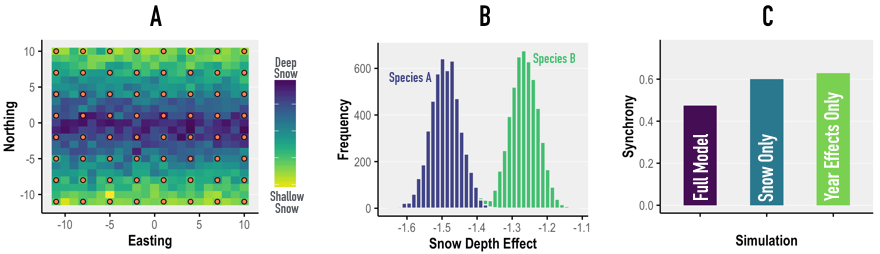
\includegraphics[width=6.5in]{./figures/figure1.png}
  \caption{An example analysis using simulated data. (A) A simulated landscape with 64 sample points and a snow depth gradient. (B) The posterior distributions of snow effects for each species ($\gamma$). Posterior estimates come from fitting the model described by equations 1-2. (C) Species synchrony, which ranges from zero (perfectly asynchronous) to one (perfectly synchronous), from model simulations where both random year effects and species-specific snow effects are included (``Full Model''), just snow effects are included (``Snow Only''), and just random year effects are included (``Year Effects Only''). In this example, both snow effects and random year effects are important for compensatory dynamics because removing them increases synchrony.}
\end{figure}

\subsection{Q2: What are the environmental drivers of observed compensatory dynamics?}

Previous research in the NWT tundra plant ecosystem shows that annual
snow depth is an important predictor of plant community composition and
population growth (Litaor et al. 2008). If species, or intraspecific
populations in different locations, have unique responses to snowdepth,
then compensatory dynamics will arise as snowdepth varies year-to-year.

I will use a flexible, dynamic spatiotemporal statistical model to
estimate species- and population-specific responses to snowdepth and
other environmental factors. As an example, consider the Saddle Grid
community at NWT, but with only two species, where snowdepth varies
across a spatial gradient and from year-to-year (Fig. 1A). We can model
species \emph{i}'s abundance (\emph{z}) at location \emph{j} and time
\emph{t} conditional on observations (\(y_{i,j,t}\)) using a Bayesian
state-space model: \vspace{-2em}

\begin{align}
y_{i,j,t} &\sim \mathcal{N}(z_{i,j,t}, \sigma_{obs.}^2), \\ 
z_{i,j,t} &\sim \mathcal{N}(\mu_{i,j,t}, \sigma_{proc.}^2), \\
\mu_{i,j,t} &= \alpha_{i,t} + \beta_{i}z_{i,j,t-1} + \gamma_{i}x_{j,t},
\end{align}\vspace{-2em}

\noindent{}where \(\mu_{i,j,t}\) is expected abundance of species
\emph{i} at location \emph{j} and time \emph{t}, \(\alpha_{i,t}\) is a
time-varying intercept for species \emph{i}, \(\beta_{i}\) is the
intraspecific density-dependence term for species \emph{i},
\(\gamma_{i}\) is the effect of snow depth for species \emph{i}, and
\(x_{j,t}\) is snow depth at location \emph{j} and time \emph{t}.
State-space models are ideal for modeling time series with missing
observations, such as the Saddle grid data, because they separate the
process (modeling \emph{z}) and the observations (conditioning on
\emph{y}).

The correlation among species' random year effects (\(\alpha\)s) and the
species-specific responses to snow depth (\(\gamma\)s) will determine
species synchrony through time. I will fit the \(\gamma\) terms
hierarchically, where the species share a mean response. If the
species-specific \(\gamma\)s (snow depth effects) do not differ, then
there is no evidence that snow depth responses determine synchrony.

As an example, I simulated data for two species sampled at 64 locations
for ten years across a snow depth gradient similar to the Saddle Grid
data (Fig. 1A). Fitting the model described in equations 1-2 shows that
random year effects are correlated, but not perfectly (posterior mean =
0.57), and that the two species have unique responses to snow depth
(Fig. 1B). I then simulated the model using random snow years to
determine the relative influence of snow depth and other environmental
factors on species synchrony (Fig. 1C).

This example averages over space, but the real analysis will not. In
fact, the process model in equation 3 will include combined
spatiotemporal effects (Conn et al. 2015) and interspecific compeition
(Farrer et al. 2014). I will use the fitted model to simulate NWT tundra
vegetation community dynamics with and without mechanisms that determine
synchrony (e.g., random year effects, species-specific responses,
population-specific responses, and random spatial effects). Doing so
will allow me to partition compensatory dynamics, and its drivers,
across levels of ecological and spatial organization.

\subsection{Q3: Will predicted climate change cause stability to increase or decrease through its affect on compensatory dynamics?}

With the fitted model from question Q2 in hand, it is straightforward to
study scenarios of climate change by altering the climate-related
covariates. Many ``what if?'' questions will be answerable, such as:

\begin{itemize}[noitemsep,nolistsep]
\item If snow depth becomes more/less variable through time and/or space, how do compensatory dynamics change?
\item Do snow depth changes mainly affect intraspecific population synchrony or species synchrony?
\item How much do compensatory dynamics across all levels impact ecosystem stability under climate change scenarios?
\end{itemize}

\noindent{}I will focus on the most relevant simulations given projected
climate changes at NWT. To identify the specific mechanisms affected by
climate change, I will take a ``leave-one-mechanism-out'' approach as
described for question Q2 for each climate change scenario. Such a
modeling exercise will pinpoint the exact level of spatial and
ecological organization at which climate change will disrupt ecosystem
stability.

\subsection{Q4: Do opposing demographic responses to climate create compensatory dynamics among populations within species?}

Local communities can fluctuate asynchronously across a landscape (beta
variability) because of species turnover (beta diversity) or
intraspecific populations responding differentially to environmental
conditions. In the latter case, the mechanism may be demographic
compensation, where individual vital rates have opposing trends across
an environmental gradient (Doak and Morris 2010). I will first
disentangle the relative effects of beta diversity and demographic
compensation on beta variability using variance partitioning and
treating rows of the Saddle Grid as replicates. Second, I will use
available demographic data to fit population-specific vital rate
regressions for focal species. I will use the randomization approach
described by Villellas et al. (2015) to statistically test for
demographic compensation. Third, I will build stochastic Integral
Projection Models using the vital rate regressions to explore the impact
of climate change on focal plant species.

\section{Roles of Fellow and Mentor}

Andrew Tredennick (the Postdoctoral Fellow) will lead all aspects of the
proposed work with input from Katharine Suding and Dan Doak (the
Mentors). Suding and Doak will provide detailed knowledge of the data
sets, study system, NWT goals. Tredennick and Suding will lead
manuscripts for questions Q1, Q2, and Q3, with input from Doak and NWT
collaborators. Tredennick and Doak will lead the manuscript for question
Q4, with input from Suding and NWT collaborators. Tredennick brings
expertise in hierarchical Bayesian modeling, dynamic population models,
and simulation approaches for gaining mechanistic insight into the
drivers of synchrony. Thus, the Fellow and Mentors are uniquely poised
to take on the proposed research.

\section{Timeline}

I (the Fellow) will begin the fellowship in July 2017. The first summer
will be spent accessing and cleaning the data set(s) and site visits to
Niwot Ridge. Subsequent semesters will be spent sequentially addressing
each research question. Benchmarks for manuscript preparation and
submission are listed below. The fellowship will end June 2019.

\footnotesize{}

\begin{longtable}[c]{@{}ll@{}}
\toprule
Time period & Goals\tabularnewline
\midrule
\endhead
Summer 2017 & Access and clean data tundra plant data; calculate
hierarchical \emph{CV}s for Q1\tabularnewline
Fall 2017 & Start fitting and simulating dynamic models for
Q2\tabularnewline
Spring 2018 & Finish analysis for Q2; write and submit first manuscript
on Q1 and Q2\tabularnewline
Summer 2018 & Start model simulations for future climate; access
demographic data; present at ESA\tabularnewline
Fall 2018 & Finish simulations for Q3 and write manuscript; begin
demographic modeling for Q4\tabularnewline
Spring 2019 & Submit Q3 manuscript; finalize demographic analysis and
begin writing manuscript\tabularnewline
Summer 2019 & Submit Q4 manuscript; shepherd papers through
review\tabularnewline
\bottomrule
\end{longtable}

\normalsize{}

\setlength{\parindent}{0ex}

\section{References}\label{references}

\footnotesize{}

Bai, Y., X. Han, J. Wu, Z. Chen, and L. Li. 2004. Ecosystem stability
and compensatory effects in the Inner Mongolia grassland. Nature
431:181--184.

Conn, P. B., D. S. Johnson, J. M. V. Hoef, M. B. Hooten, J. M. London,
and P. L. Boveng. 2015. Using spatiotemporal statistical models to
estimate animal abundance and infer ecological dynamics from survey
counts. Ecological Monographs 85:235--252.

Doak, D. F., and W. F. Morris. 2010. Demographic compensation and
tipping points in climate-induced range shifts. Nature 467:959--962.

Farrer, E. C., I. W. Ashton, J. Knape, and K. N. Suding. 2014.
Separating direct and indirect effects of global change: a population
dynamic modeling approach using readily available field data. Global
change biology 20:1238--50.

Gonzalez, A., and M. Loreau. 2009. The Causes and Consequences of
Compensatory Dynamics in Ecological Communities. Annual Review of
Ecology, Evolution, and Systematics 40:393--414.

Litaor, M. I., M. Williams, and T. R. Seastedt. 2008. Topographic
controls on snow distribution, soil moisture, and species diversity of
herbaceous alpine Vegetation, Niwot Ridge, Colorado. Journal of
Geophysical Research: Biogeosciences 113.

Loreau, M., and C. {{de Mazancourt}}. 2008. Species synchrony and its
drivers: neutral and nonneutral community dynamics in fluctuating
environments. The American Naturalist 172:E48--E66.

Loreau, M., and C. {{de Mazancourt}}. 2013. Biodiversity and ecosystem
stability: A synthesis of underlying mechanisms. Ecology Letters
16:106--115.

Villellas, J., D. F. Doak, M. B. Garc{í}a, and W. F. Morris. 2015.
Demographic compensation among populations: what is it, how does it
arise and what are its implications? Ecology Letters 18:1139--1152.

Wang, S., and M. Loreau. 2014. Ecosystem stability in space: \(\alpha\),
\(\beta\) and \(\gamma\) variability. Ecology Letters 17:891--901.

Wang, S., and M. Loreau. 2016. Biodiversity and ecosystem stability
across scales in metacommunities. Ecology Letters 19:510--518.

\end{document}
